\documentclass[12pt,a4paper]{article}
% Estilo compartido para informes. Compilar con LuaLaTeX desde tp1/.
\usepackage[spanish,es-nodecimaldot]{babel}
\usepackage{fontspec}
\setmainfont{Montserrat-Medium.ttf}[
  Path=../assets/fonts/,
  BoldFont=Montserrat-Bold.ttf,
  ItalicFont=Montserrat-MediumItalic.ttf]
\usepackage[a4paper,margin=2.5cm,headheight=16pt]{geometry}
\usepackage{xcolor,graphicx,booktabs,tabularx}
\usepackage{float}
\usepackage{titlesec,fancyhdr,enumitem,caption}
\usepackage{ragged2e}
\usepackage{hyperref}
\definecolor{verde}{HTML}{1D4036}
\definecolor{bronce}{HTML}{D38129}
\definecolor{rosa}{HTML}{D88E77}
\definecolor{calido}{HTML}{EFE4D8}
\definecolor{grafito}{HTML}{1D1D1D}
\hypersetup{colorlinks=true,linkcolor=verde,urlcolor=verde,
  pdftitle={TP1 - Instalación de máquinas virtuales},pdfsubject={Cyberseguridad}}
\AtBeginDocument{\color{grafito}\RaggedRight\fontsize{12}{14.4}\selectfont}
\setlength{\parindent}{0pt}
\setlength{\parskip}{7pt}
\setlist[itemize]{leftmargin=*,itemsep=7pt,topsep=4pt}
\setlist[enumerate]{leftmargin=*,itemsep=6pt}
\titleformat{\section}{\color{verde}\bfseries\fontsize{18}{21.6}\selectfont}{\thesection}{0.65em}{}
\titleformat{\subsection}{\color{verde}\bfseries\large}{\thesubsection}{0.65em}{}
\titleformat{\subsubsection}{\color{verde}\bfseries}{\thesubsubsection}{0.65em}{}
\titlespacing*{\section}{0pt}{16pt}{8pt}
\titlespacing*{\subsection}{0pt}{12pt}{5pt}
\titlespacing*{\subsubsection}{0pt}{10pt}{4pt}
\setcounter{tocdepth}{2}
\pagestyle{fancy}
\fancyhf{}
\fancyhead[L]{\small\color{verde}FCEFyN | UNC}
\fancyhead[R]{\small\color{verde}\materia\ · TP \numeroTP}
\fancyfoot[L]{\scriptsize Informe de laboratorio}
\fancyfoot[R]{\small\thepage}
\renewcommand{\headrulewidth}{0.4pt}
\captionsetup{font=small,labelfont=bf,justification=raggedright,singlelinecheck=false,hypcap=false}
\newcommand{\pendiente}[1]{\par{\small\color{verde}\textbf{Por completar.} #1\par}}
% Si falta una captura se muestra un espacio reservado; no impide compilar.
\newcommand{\captura}[2]{%
  \par\smallskip\begingroup\centering
  \IfFileExists{figuras/#1}{%
    \includegraphics[width=\linewidth,height=5cm,keepaspectratio]{figuras/#1}%
  }{%
    \setlength{\fboxsep}{10pt}%
    \fcolorbox{bronce}{calido}{\parbox[c][1.25cm][c]{\dimexpr\linewidth-2\fboxsep-2\fboxrule\relax}{%
      \centering\small Captura pendiente\par\texttt{\detokenize{#1}}}}%
  }%
  \captionof{figure}{#2}\par\endgroup\smallskip
}


\newcommand{\materia}{Cyberseguridad}
\newcommand{\numeroTP}{1}
\newcommand{\tituloTP}{Instalación de máquinas virtuales}
\newcommand{\estudiante}{Brigido Tomas Andres}
\newcommand{\legajo}{38481096}
\newcommand{\carrera}{ICOMP}
\newcommand{\docente}{Javier A. Jorge}


\begin{document}
\hypersetup{pageanchor=false}
\begin{titlepage}
  
\includegraphics[width=8cm]{../assets/logo-fcefyn-2026.png}
  \vspace{1cm}

  {\color{verde}\small UNIVERSIDAD NACIONAL DE CÓRDOBA\par}
  \vspace{2.1cm}
  {\color{bronce}\bfseries\large TRABAJO PRÁCTICO \numeroTP\par}
  \vspace{0.45cm}
  {\color{verde}\bfseries\fontsize{32}{38.4}\selectfont Instalación de\\máquinas virtuales\par}
  \vspace{0.65cm}
  {\large \materia\par}
  \vspace{0.8cm}
  {\color{bronce}\rule{2.7cm}{2pt}\par}
  \vfill
  \renewcommand{\arraystretch}{1.45}
  \begin{tabular}{@{}p{3.2cm}p{10cm}@{}}
    Estudiante & \estudiante \\
    Legajo & \legajo \\
    Carrera & \carrera \\
    Docente & \docente \\
  \end{tabular}
  \vfill
  {\small Córdoba, Argentina\par}
\end{titlepage}
\hypersetup{pageanchor=true}

\tableofcontents
\vspace{1cm}
\newpage

\section{Introducción y objetivos}
Este trabajo toma como referencia la práctica de laboratorio 1.1.5 de Cisco Networking Academy, orientada a preparar un entorno virtual para las actividades de la materia. La consigna contempla la instalación de VirtualBox y la importación de las imágenes CyberOps Workstation y Security Onion.

\subsection{Objetivos}
\begin{itemize}
  \item Preparar la computadora anfitriona para ejecutar máquinas virtuales.
  \item Importar las imágenes del curso al inventario de VirtualBox.
  \item Iniciar CyberOps Workstation, explorar sus herramientas y comprobar la conectividad.
  \item Registrar el cierre del entorno y reflexionar sobre el uso de la virtualización.
\end{itemize}

\section{Desarrollo de la práctica}
\subsection{Parte 1: preparación del anfitrión}
\subsubsection{Instalación de VirtualBox}
Como primera medida se descargaron las imagenes de VirtualBox y de las máquinas virtuales desde el sitio oficial de Cisco Networking Academy. Luego se procedió a instalar VirtualBox en la computadora anfitriona siguiendo los pasos del instalador.
\begin{figure}[htbp]
    \centering
    \begin{minipage}[t]{0.48\textwidth}
        \centering
        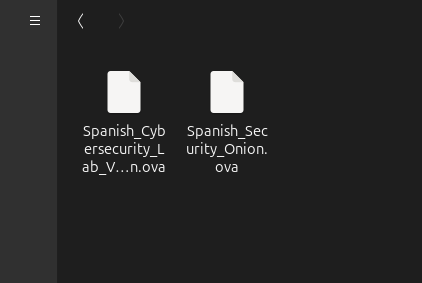
\includegraphics[width=\linewidth]{img/VMimgs.png}
        \caption{Imagenes de las máquinas virtuales.}
        \label{fig:imagen1}
    \end{minipage}
    \hfill
    \begin{minipage}[t]{0.48\textwidth}
        \centering
        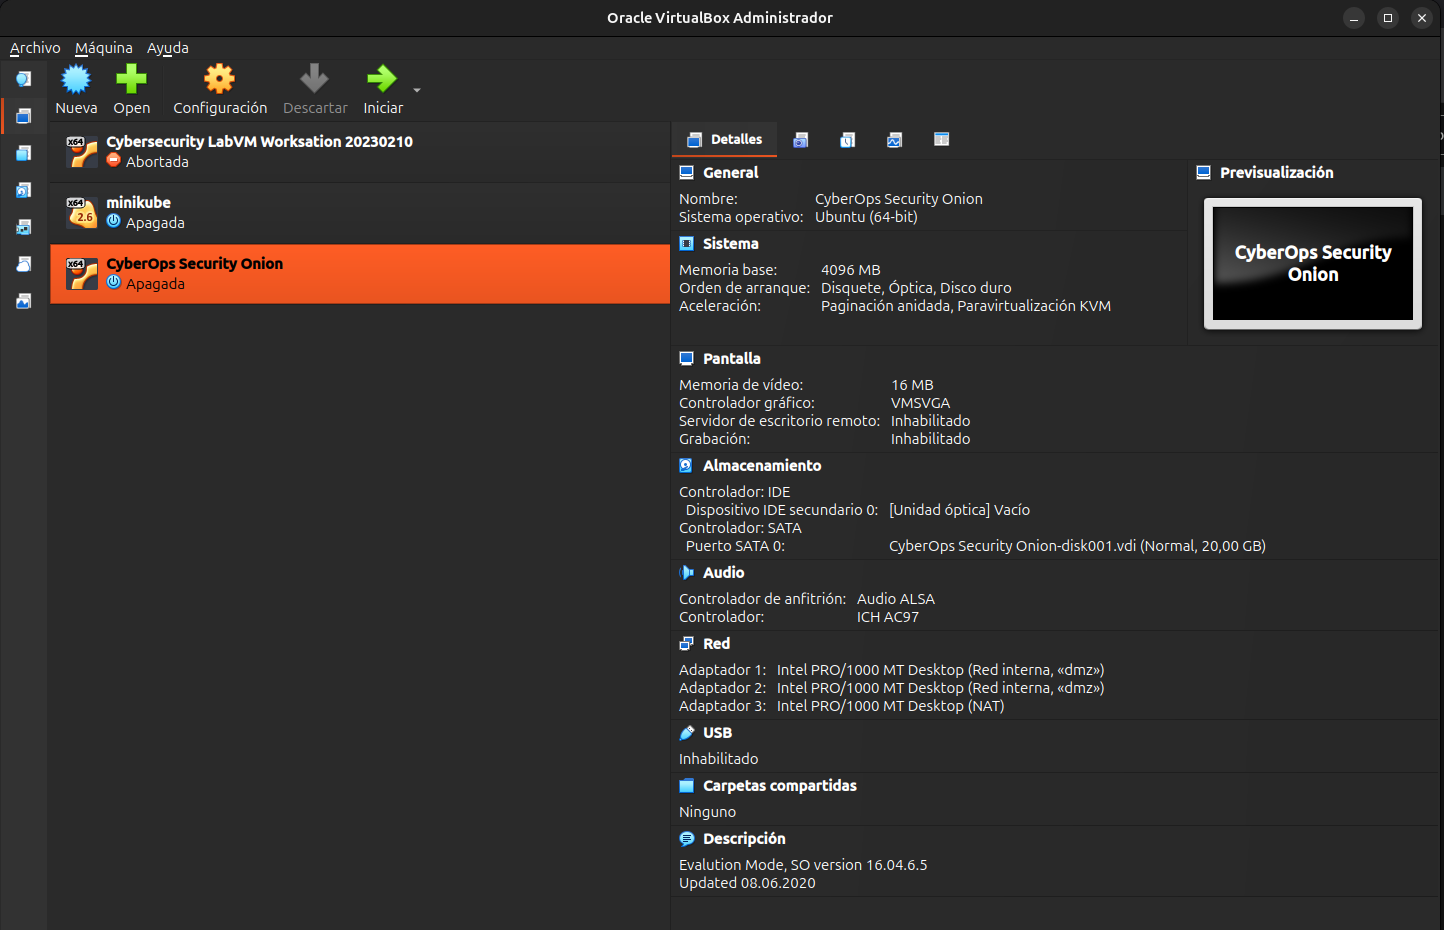
\includegraphics[width=\linewidth]{img/VMinstaladas.png}
        \caption{Máquinas virtuales instaladas en VirtualBox.}
        \label{fig:imagen2}
    \end{minipage}
\end{figure}

\subsubsection{Inicio y acceso a CyberOps Workstation y aplicaciones}
Luego de importar la imagen de CyberOps Workstation, se inició la máquina virtual y se comprobó que las aplicaciones de CyberOps Workstation se encontraban disponibles.
Las aplicaciones disponibles son IDLE, SciTe Text Editor y Wireshark.
\begin{figure}[H]
    \centering
    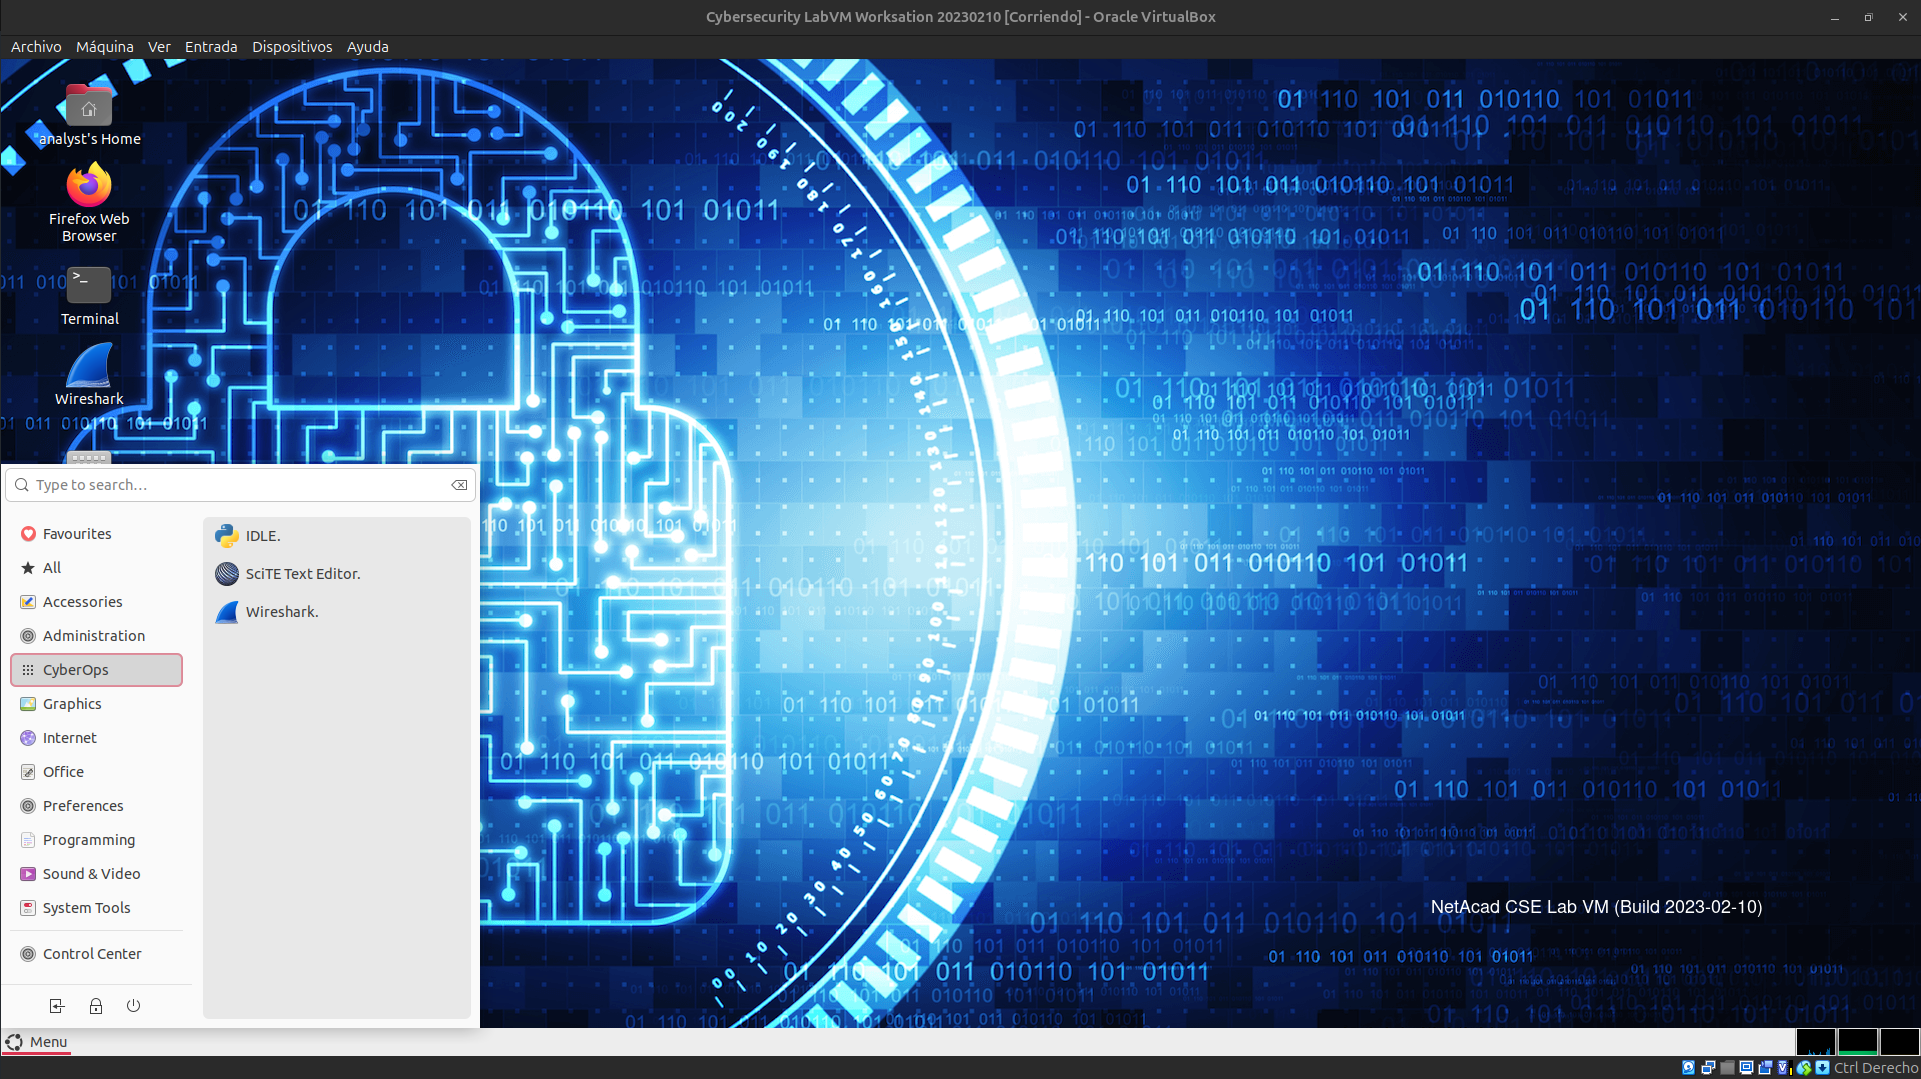
\includegraphics[width=0.85\textwidth]{img/mviniciada.png}
    \caption{Máquina virtual iniciada.}
    \label{fig:mi-imagen}
\end{figure}

\subsubsection{Direcciones IP y conectividad}

\begin{figure}[H]
    \centering
    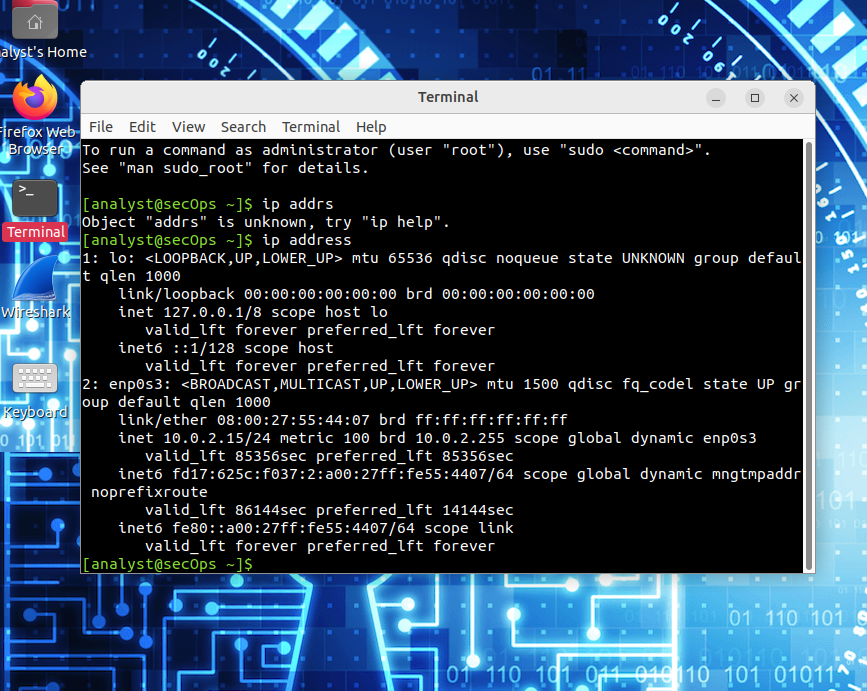
\includegraphics[width=0.75\textwidth]{img/ipaddress.png}
    \caption{Direcciones IP de la máquina virtual.}
    \label{fig:mi-imagen}
\end{figure}

El comando \texttt{ip address} muestra las interfaces de red de la VM.
Los bloques \texttt{1:} y \texttt{2:} identifican interfaces distintas.
\begin{itemize}
    \item \textbf{\texttt{1: lo} (loopback):} es la interfaz interna que
    permite que los programas de la VM se comuniquen dentro de la misma
    máquina, sin salir a la red. Sus direcciones son \texttt{127.0.0.1}
    en IPv4 y \texttt{::1} en IPv6.
    \item \textbf{\texttt{2: enp0s3}:} es la tarjeta de red virtual que
    conecta la VM con la red proporcionada por VirtualBox. Tiene asignada
    la IPv4 \texttt{10.0.2.15}. Las líneas \texttt{inet6} muestran sus
    direcciones IPv6 y \texttt{link/ether} indica su dirección MAC.
\end{itemize}
Cada interfaz puede tener varias direcciones. La IPv4 de la VM para
comunicarse por la red es \texttt{10.0.2.15}, correspondiente a
\texttt{enp0s3}.

\subsubsection{Cierre de las máquinas virtuales}
En esta seccion se utilizo el comando \texttt{shutdown} para apagar la máquina virtual de manera segura. Esto asegura que todos los procesos se cierren correctamente y que no haya pérdida de datos.
No me parecio que aporte mucho al informe integrar capturas de este comando pero se puedo realizar exitosamente.

\section{Reflexión}
\textbf{¿Cuáles son las ventajas y desventajas de usar una máquina virtual?}
Una de las principales ventajas de utilizar una máquina virtual es la seguridad que te da tener ese entorno cerrado
a la hora de probar software desconocido.
Si hay algun archivo del cual desconfio pensaria primero en descargarlo y ejecutarlo
en una maquina virtual para asegurarme que no sea malicioso y no afecte mi computadora anfitriona.

No haria mencion al tema de la portabilidad o modularidad que se puede llegar con una maquina virtual ya que hoy en dia existen
herramientas como Docker que permiten tener un entorno aislado y portable sin necesidad de virtualizar todo un sistema operativo.

\newpage
\section{Referencias}
\begin{enumerate}
  \item Cisco Networking Academy. \textit{Práctica de laboratorio: Instalar las máquinas virtuales}, actividad 1.1.5, 2018--2020. Consigna suministrada en el archivo \nolinkurl{1.1.5-lab---installing-the-virtual-machines_es-XL.pdf}.
  \item FCEFyN, Universidad Nacional de Córdoba. \textit{Manual de identidad visual}, 2026. Material proporcionado en la carpeta \texttt{assets}; pautas de marca, color y tipografía, pp. 11--22.
\end{enumerate}

\end{document}
